\documentclass{article}

\usepackage{fancyhdr}
\usepackage{extramarks}
\usepackage{minted}
\usepackage[T1]{fontenc}
\usepackage{graphicx}
\usepackage{inconsolata}
\usepackage{multicol}
\usepackage{enumitem}
\usepackage{tikz}
\usetikzlibrary{positioning}

\tikzset{
  gray box/.style={
    fill=gray!20,
    draw=gray,
    minimum width={2*#1ex},
    minimum height={2em},
  },
  annotation/.style={
    anchor=north,
  }
}


%
% Basic Document Settings
%

\topmargin=-0.45in
\evensidemargin=0in
\oddsidemargin=0in
\textwidth=6.5in
\textheight=9.0in
\headsep=0.25in

\linespread{1.1}

\pagestyle{fancy}
\lhead{\hmwkAuthorName}
\chead{\hmwkClass: \hmwkTitle}
\rhead{\firstxmark}
\lfoot{\lastxmark}
\cfoot{\thepage}

\renewcommand\headrulewidth{0.4pt}
\renewcommand\footrulewidth{0.4pt}

\setlength\parindent{0pt}

%
% Create Problem Sections
%

\newcommand{\enterProblemHeader}[1]{
\nobreak\extramarks{}{Problem \arabic{#1} continued on next page\ldots}\nobreak{}
\nobreak\extramarks{Problem \arabic{#1} (continued)}{Problem \arabic{#1} continued on next page\ldots}\nobreak{}
}

\newcommand{\exitProblemHeader}[1]{
\nobreak\extramarks{Problem \arabic{#1} (continued)}{Problem \arabic{#1} continued on next page\ldots}\nobreak{}
\stepcounter{#1}
\nobreak\extramarks{Problem \arabic{#1}}{}\nobreak{}
}

\setcounter{secnumdepth}{0}
\newcounter{partCounter}
\newcounter{homeworkProblemCounter}
\setcounter{homeworkProblemCounter}{1}
\nobreak\extramarks{Problem \arabic{homeworkProblemCounter}}{}\nobreak{}

%
% Homework Problem Environment
%
% This environment takes an optional argument. When given, it will adjust the
% problem counter. This is useful for when the problems given for your
% assignment aren't sequential. See the last 3 problems of this template for an
% example.
%
\newenvironment{homeworkProblem}[1][-1]{
\ifnum#1>0
\setcounter{homeworkProblemCounter}{#1}
\fi
\section{Problem \arabic{homeworkProblemCounter}}
\setcounter{partCounter}{1}
\enterProblemHeader{homeworkProblemCounter}
}{
\exitProblemHeader{homeworkProblemCounter}
}

%
% Homework Details
%   - Title
%   - Due date
%   - Class
%   - Section/Time
%   - Instructor
%   - Author
%

\newcommand{\hmwkTitle}{Homework\ \#3}
\newcommand{\hmwkDueDate}{March 1, 2016}
\newcommand{\hmwkClass}{Operating Systems}
\newcommand{\hmwkClassTime}{Monday \& Wednesday 3:30pm --- 5:17pm}
\newcommand{\hmwkClassInstructor}{Professor Qu}
\newcommand{\hmwkAuthorName}{Nicholas Land}

%
% Title Page
%

\title{
\vspace{2in}
\textmd{\textbf{\hmwkClass:\ \hmwkTitle}}\\
\normalsize\vspace{0.1in}\small{Due\ on\ \hmwkDueDate\ at 11:59pm}\\
\vspace{0.1in}\large{\textit{\hmwkClassInstructor\ \\ \hmwkClassTime}}
\vspace{3in}
}

\author{\textbf{\hmwkAuthorName}}
\date{}

\renewcommand{\part}[1]{\textbf{\large Part \Alph{partCounter}}\stepcounter{partCounter}\\}

%
% Various Helper Commands
%

% Alias for the Solution section header
\newcommand{\solution}{\textsc{\textbf Solution}\\}

% Alias for bold small caps
\newcommand{\smallcaps}[1]{\textsc{\textbf #1}\\}

\begin{document}

  \maketitle

  \pagebreak

  \begin{homeworkProblem}

    Consider the following process arrival list:

    \begin{center}
      \begin{tabular}{c c c}
        \underline{Name} & \underline{Arrival time} & \underline{Service time} \\
        A & $0$ & $4$ \\
        B & $3$ & $9$ \\
        C & $5$ & $2$ \\
        D & $7$ & $5$ \\
        E & $11$ & $3$ \\
        F & $13$ & $1$ \\
        G & $21$ & $4$ \\
      \end{tabular}
    \end{center}

    Consider the following scheduling methods:

    \begin{multicols}{2}
      \begin{enumerate}[label=(\alph*)]
        \item First-come first-served (FCFS)
        \item Shortest-job first (SJF)
        \vfill
        \columnbreak
        \item Shortest remaining time first (SRTF)
        \item Round-robin (RR), Quantum = 5
      \end{enumerate}
    \end{multicols}

    Draw a Gantt chart (time line) showing which process is executing over time and calculate the average waiting time and average completion time. \\

    Notes : (1) In SRTF, if a process arrives with service time equal to the remaining service time of the process currently being served, the current process is not interrupted. (2) In RR, if a process arrives at the same time a quantum finishes, the running process is preempted and the new arrival executes.  The preempted process goes to the end of the ready queue. (3) Waiting time and completion time is defined as in the slides. \\

    \solution

    \begin{center}
      \smallcaps{(a) First-come first-served (FCFS)}
      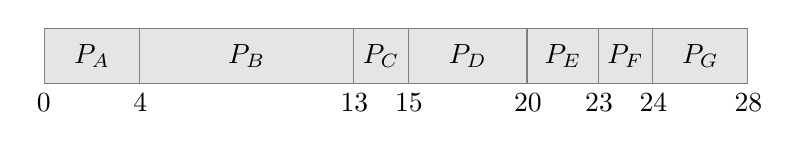
\begin{tikzpicture}[node distance=-0.5pt]
        \node [gray box=4] (p1) {\(P_{A}\)};
        \node [gray box=9, right=of p1] (p2) {\(P_{B}\)};
        \node [gray box=2, right=of p2] (p3) {\(P_{C}\)};
        \node [gray box=5, right=of p3] (p4) {\(P_{D}\)};
        \node [gray box=3, right=of p4] (p5) {\(P_{E}\)};
        \node [gray box=1, right=of p5] (p6) {\(P_{F}\)};
        \node [gray box=4, right=of p6] (p7) {\(P_{G}\)};

        \node [annotation] at (p1.south west) {0};
        \node [annotation] at (p1.south east) {4};
        \node [annotation] at (p2.south east) {13};
        \node [annotation] at (p3.south east) {15};
        \node [annotation] at (p4.south east) {20};
        \node [annotation] at (p5.south east) {23};
        \node [annotation] at (p6.south east) {24};
        \node [annotation] at (p7.south east) {28};
      \end{tikzpicture}

      \textbf{Average waiting time:} $(0 + 1 + 8 + 8 + 9 + 10 + 3) \div 7 = 5.6$ \\
      \textbf{Average completion time:} $(4 + 10 + 10 + 13 + 12 + 11 + 7) \div 7 = 9.6$
    \end{center}

    \begin{center}
      \smallcaps{(b) Shortest-job first (SJF)}
      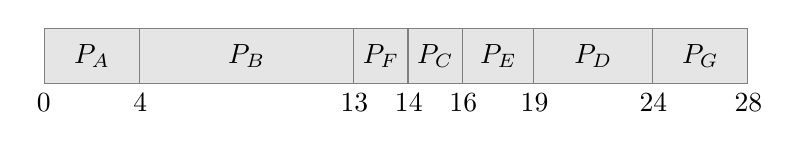
\begin{tikzpicture}[node distance=-0.5pt]
        \node [gray box=4] (p1) {\(P_{A}\)};
        \node [gray box=9, right=of p1] (p2) {\(P_{B}\)};
        \node [gray box=1, right=of p2] (p3) {\(P_{F}\)};
        \node [gray box=2, right=of p3] (p4) {\(P_{C}\)};
        \node [gray box=3, right=of p4] (p5) {\(P_{E}\)};
        \node [gray box=5, right=of p5] (p6) {\(P_{D}\)};
        \node [gray box=4, right=of p6] (p7) {\(P_{G}\)};

        \node [annotation] at (p1.south west) {0};
        \node [annotation] at (p1.south east) {4};
        \node [annotation] at (p2.south east) {13};
        \node [annotation] at (p3.south east) {14};
        \node [annotation] at (p4.south east) {16};
        \node [annotation] at (p5.south east) {19};
        \node [annotation] at (p6.south east) {24};
        \node [annotation] at (p7.south east) {28};
      \end{tikzpicture}

      \textbf{Average waiting time:} $(0 + 1 + 9 + 12 + 5 + 0 + 3)
      \div 7 = 4.2$ \\
      \textbf{Average completion time:} $(4 + 10 + 11 + 17 + 8 + 1 + 7) \div 7 = 8.3$
    \end{center}

    \begin{center}
      \smallcaps{(c) Shortest remaining time first {SRTF}}
      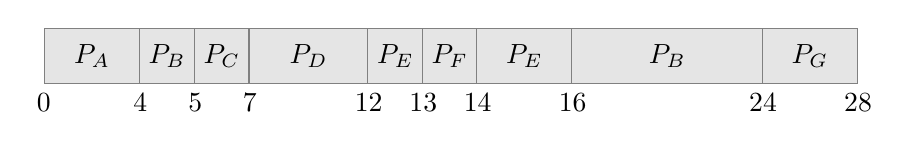
\begin{tikzpicture}[node distance=-0.5pt]
        \node [gray box=4] (p1) {\(P_{A}\)};
        \node [gray box=1, right=of p1] (p2) {\(P_{B}\)};
        \node [gray box=2, right=of p2] (p3) {\(P_{C}\)};
        \node [gray box=5, right=of p3] (p4) {\(P_{D}\)};
        \node [gray box=1, right=of p4] (p5) {\(P_{E}\)};
        \node [gray box=1, right=of p5] (p6) {\(P_{F}\)};
        \node [gray box=4, right=of p6] (p7) {\(P_{E}\)};
        \node [gray box=8, right=of p7] (p8) {\(P_{B}\)};
        \node [gray box=4, right=of p8] (p9) {\(P_{G}\)};

        \node [annotation] at (p1.south west) {0};
        \node [annotation] at (p1.south east) {4};
        \node [annotation] at (p2.south east) {5};
        \node [annotation] at (p3.south east) {7};
        \node [annotation] at (p4.south east) {12};
        \node [annotation] at (p5.south east) {13};
        \node [annotation] at (p6.south east) {14};
        \node [annotation] at (p7.south east) {16};
        \node [annotation] at (p8.south east) {24};
        \node [annotation] at (p9.south east) {28};
      \end{tikzpicture}

      \textbf{Average waiting time:} $(0 + 12 + 0 + 0 + 2 + 0 + 3) \div 7 = 2.4$ \\
      \textbf{Average completion time:} $(4 + 21 + 2 + 5 + 5 + 1 + 7) \div 7 = 6.4$
    \end{center}

    \begin{center}
      \smallcaps{(d) Round-robin, Quantum = 5}
      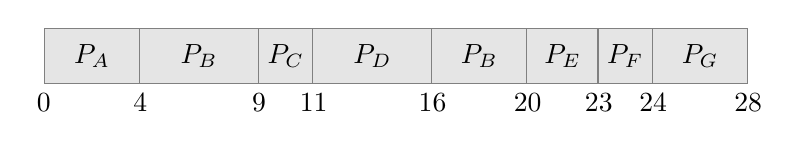
\begin{tikzpicture}[node distance=-0.5pt]
        \node [gray box=4] (p1) {\(P_{A}\)};
        \node [gray box=5, right=of p1] (p2) {\(P_{B}\)};
        \node [gray box=2, right=of p2] (p3) {\(P_{C}\)};
        \node [gray box=5, right=of p3] (p4) {\(P_{D}\)};
        \node [gray box=4, right=of p4] (p5) {\(P_{B}\)};
        \node [gray box=3, right=of p5] (p6) {\(P_{E}\)};
        \node [gray box=1, right=of p6] (p7) {\(P_{F}\)};
        \node [gray box=4, right=of p7] (p8) {\(P_{G}\)};

        \node [annotation] at (p1.south west) {0};
        \node [annotation] at (p1.south east) {4};
        \node [annotation] at (p2.south east) {9};
        \node [annotation] at (p3.south east) {11};
        \node [annotation] at (p4.south east) {16};
        \node [annotation] at (p5.south east) {20};
        \node [annotation] at (p6.south east) {23};
        \node [annotation] at (p7.south east) {24};
        \node [annotation] at (p8.south east) {28};
      \end{tikzpicture}

      \textbf{Average waiting time:} $(0 + 8 + 4 + 4 + 9 + 10 + 3) \div 7 = 5.4$ \\
      \textbf{Average completion time:} $(4 + 17 + 6 + 9 + 12 + 11 + 7) \div 7 = 9.4$
    \end{center}
  \end{homeworkProblem}

  \begin{homeworkProblem}
    A Multilevel feedback queues are shown in the diagram below. The scheduler first executes all processes in Q0. Only when Q0 is empty will it execute processes in Q1, and only when Q0 and Q1 are empty will it execute processes in Q2. A process arriving for Q0 will preempt a process in Q1 or Q2, and a process arriving for Q1 will preempt a process in Q2; a process preempted in this case is put back to the head of the same queue; when this process is scheduled to run next time it will execute for the remaining of its allocated time quantum. A new process entering the system is put in Q0 and is given a time quantum of 8 milliseconds. If it does not finish within this time, it is preempted and moved to the tail of Q1. If Q0 is empty, the process at the head of Q1 is scheduled to run with a time quantum of 16 milliseconds. If it does not finish within this time, it is preempted and moved to the tail of Q2. Processes in Q2 are run on an FCFS basis. \\

    \begin{center}
      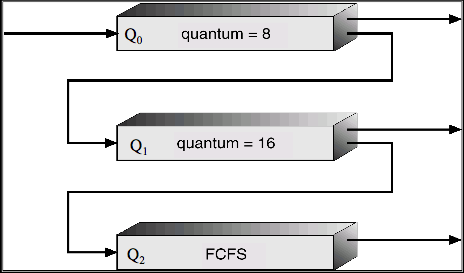
\includegraphics[scale=0.5]{image.png} \\
    \end{center}

    Given the following arrival time and CPU burst of processes A, B, C, D, and E as shown in table below.

    \begin{center}
      \begin{tabular}{ | c | c | c |}
        \hline
        Task & Arrival Time & Service Time \\
        \hline
        A & 0 & 25 \\
        \hline
        B & 5 & 28 \\
        \hline
        C & 19 & 11 \\
        \hline
        D & 25 & 19 \\
        \hline
        E & 36 & 33 \\
        \hline
      \end{tabular}
    \end{center}

    \begin{enumerate}[label=\alph*)]
      \item Show the status of each queue along the time line during the running of the system. You only need to show the status of the system when either 1) a new process arrives, or 2) a process is preempted, or 3) a process terminates. The status includes time stamp, the name of the process and its remaining time in each queue. For example, at time 0, process A is in $Q_0$ and it has 25 time units toward finishing. $Q_1$ and $Q_2$ are empty. You are asked to complete the table with time moment and status of each queue. Moreover, B(x) A(y) shows A is at the head of the queue with x remaining time and B is at the tail of the queue with remaining time of y. You can add new rows to the table if you think the table is not enough to accommodate all the events.
    \end{enumerate}

    \solution

    \begin{center}
      \begin{tabular}{| c | c | c | c |}
        \hline
        \textbf{Time} & $Q_0$ & $Q_1$ & $Q_2$ \\
        \hline
        0 & A(25) & &  \\
        \hline
        5 & B(28) A(20) & & \\
        \hline
        8 & B(28) & A(17) & \\
        \hline
        16 & & A(17) B(20) & \\
        \hline
        19 & C(11) & A(14) B(20) & \\
        \hline
        25 & C(5) D(19) & A(14) B(20) & \\
        \hline
        27 & D(19) & A(14) B(20) C(3) & \\
        \hline
        35 & & A(14) B(20) C(3) D(11) & \\
        \hline
        36 & E(33) & A(13) B(20) C(3) D(11) & \\
        \hline
        44 & & A(13) B(20) C(3) D(11) E(25) & \\
        \hline
        56 & & B(20) C(3) D(11) E(25) & A(1) \\
        \hline
        72 & & C(3) D(11) E(25) & A(1) B(4) \\
        \hline
        75 & & Process C terminates D(11) E(25) & A(1) B(4) \\
        \hline
        86 & & Process D terminates E(25) & A(1) B(4) \\
        \hline
        102 & & & A(1) B(4) E(9) \\
        \hline
        103 & & & Process A terminates B(4) E(9) \\
        \hline
        107 & & & Process B terminates E(9) \\
        \hline
        116 & & & Process E terminates \\
        \hline
      \end{tabular}
    \end{center}
  \end{homeworkProblem}

\end{document}
